\section{算子范数}
\label{sec:lop-operator-norm}

输入$x$带上扰动$e$以后，线性算子的输出变为$T(x+e)=Tx+Te$。输出误差$Te$只取决于扰动本身，与$x$在哪里无关。于是“误差会被放大多少”化为一个问题：能否找到一个常数，控制一切扰动经过$T$后的大小？

对矩阵，这个问题总有答案。单位球是紧集，$\lVert\bm A\bm x\rVert$连续，最大值一定取到。算子没有这样的保证：单位球不紧，放大倍数可能无穷大。本节先用一个统一不等式定义有界性，再通过求导和积分说明条件的作用，最后定义算子范数。

\subsection{算子的有界性}
\label{sec:lop-boundedness}

下面设$X,Y$是赋范空间，$T:D(T)\to Y$是线性算子，$D(T)\subseteq X$沿用$X$的范数，$Y$使用它自己的范数。我们希望用一个与输入无关的常数$C$控制$\lVert Tx\rVert$，这样输入误差为$\lVert e\rVert$时，输出误差不超过$C\lVert e\rVert$。

\begin{definition}[有界线性算子]
\label{def:lop-bounded-operator}
若存在常数$C\geq0$，使
\begin{equation}
 \lVert Tx\rVert_Y\leq C\lVert x\rVert_X\qquad(x\in D(T)),
 \label{eq:lop-bounded}
\end{equation}
则称线性算子$T$为\term{有界线性算子}（bounded linear operator），简称有界算子。不存在这样的常数时，称$T$为\term{无界算子}（unbounded operator）。
\end{definition}

这里的“有界”说的是输出与输入之比有统一上界，不是说输出集合$\{Tx:x\in D(T)\}$有界：非零线性算子的像在数乘下封闭，总是无界集合。条件~\eqref{eq:lop-bounded}也可以只在单位球上检查。按线性把$x\neq0$缩放为$x/\lVert x\rVert$，它等价于
\[
 \sup\{\lVert Tx\rVert:x\in D(T),\ \lVert x\rVert\leq1\}<\infty.
\]

第~\ref{chap:metric-space-maps}章在度量空间之间定义了连续映射与Lipschitz映射：后者要求存在常数$L$使输出距离不超过$L$倍的输入距离，它比连续更强。对一般映射，二者相差很远；对线性算子，下面的定理说明它们与有界性是一回事。

\begin{theorem}[有界与连续等价]
\label{thm:lop-bounded-continuous}
对赋范空间之间的线性算子$T:D(T)\to Y$，下列四条等价：（i）$T$在$0$处连续；（ii）$T$在$D(T)$上处处连续；（iii）$T$是Lipschitz映射；（iv）$T$有界。
\end{theorem}

\begin{proof}
若（iv）成立，由线性，
\[
 \lVert Tx-Tz\rVert=\lVert T(x-z)\rVert\leq C\lVert x-z\rVert,
\]
这就是（iii）。Lipschitz映射处处连续，故（iii）推出（ii）；处处连续自然包含在$0$处连续，故（ii）推出（i）。

只需再证（i）推出（iv）。取$\varepsilon=1$，由$T$在$0$处连续及$T0=0$，存在$\delta>0$，使$x\in D(T)$且$\lVert x\rVert\leq\delta$时$\lVert Tx\rVert\leq1$。

对任意$x\neq0$，向量$\delta x/\lVert x\rVert$的范数为$\delta$，于是
\[
 \lVert Tx\rVert=\frac{\lVert x\rVert}{\delta}\Bigl\lVert T\Bigl(\frac{\delta x}{\lVert x\rVert}\Bigr)\Bigr\rVert\leq\frac{1}{\delta}\lVert x\rVert .
\]
取$C=1/\delta$即得（iv）。
\end{proof}

证明的关键是缩放：线性算子在零点附近一个小球上的行为，决定了它在所有尺度上的行为。有限维空间中所有范数等价，线性映射总是有界的；无限维中这一点不再自动成立，下面两个例子分别给出失败与成立的情形。

\subsubsection{有界性依赖定义域范数}
\label{sec:lop-derivative-boundedness}

求导的“矩阵”先用差分看清楚。在$[0,1]$上取$n+1$个等距点，步长$h=1/n$，差分$(f_{i+1}-f_i)/h$就是一行只有两个非零元素$\pm1/h$的矩阵。网格加细时，矩阵元素按$1/h$增大。

取输入为交错序列$f_i=(-1)^i$，它的每个分量绝对值都是$1$，输出的每个分量绝对值都是$2/h=2n$。例如$h=1/4$时，输入$(1,-1,1,-1,1)$的输出是$(-8,8,-8,8)$。网格越细，这个矩阵的放大倍数越大，极限下不存在上界。积分的矩阵正好相反，元素里带一个小因子$h$。

现在回到连续的情形。考虑求导$D:C^1[0,1]\to C[0,1]$，$Df=f^\prime$，取值空间始终使用一致范数$\lVert g\rVert_\infty=\max_{[0,1]}\lvert g\rvert$。先在定义域上使用同时计入函数值与导数的范数
\[
 \lVert f\rVert_{C^1}=\lVert f\rVert_\infty+\lVert f^\prime\rVert_\infty .
\]
这时
\[
 \lVert Df\rVert_\infty=\lVert f^\prime\rVert_\infty\leq\lVert f\rVert_{C^1},
\]
取$C=1$即满足式~\eqref{eq:lop-bounded}，$D$是有界算子。

再在同一个函数集合$C^1[0,1]$上只用一致范数衡量输入。取$f_n(x)=\sin(2\pi nx)$，则
\[
 \lVert f_n\rVert_\infty=1,\qquad \lVert Df_n\rVert_\infty=\lVert2\pi n\cos(2\pi nx)\rVert_\infty=2\pi n .
\]
输出与输入的范数之比为$2\pi n$，随$n$无界增长，不存在统一常数，$D$是无界算子。振幅不变而频率升高时，函数值始终在$[-1,1]$中，斜率却按频率放大；一个一致范数很小的高频扰动$\varepsilon f_n$，可以使导数产生$2\pi n\varepsilon$的误差。

两种情形中，求导公式与允许的函数集合都没有变，变化的只是定义域上的范数。所以说一个算子是否有界，必须同时交代作用规则、定义域和两侧的范数。前一种范数把导数的大小也算进输入的“大小”，因而能控制输出；后一种范数看不见导数，也就无从控制它。

两种范数的另一个差别是完备性。只配一致范数的$C^1[0,1]$不是Banach空间。函数$g_n(x)=\sqrt{(x-1/2)^2+n^{-2}}$都连续可导，并且
\[
 0\leq g_n(x)-\lvert x-\tfrac12\rvert=\frac{n^{-2}}{g_n(x)+\lvert x-1/2\rvert}\leq\frac1n,
\]
所以$(g_n)$按一致范数收敛到不可导的$\lvert x-1/2\rvert$，是$C^1[0,1]$中没有极限的柯西列。

第~\ref{sec:lop-fundamental-theorems}节的算子定理都要求Banach空间，因此不能直接套用在这样的定义域上。配上$\lVert\cdot\rVert_{C^1}$后，$C^1[0,1]$是完备的（第~\ref{sec:lop-closed-graph}小节用积分表示说明这一点），那些定理才能使用。

\subsubsection{积分算子的有界性}
\label{sec:lop-integral-bounded}

现在回到积分变换~\eqref{eq:lop-integral-operator}。先看矩阵的情形。输出的第$i$个分量是第$i$行与输入的内积，由Cauchy--Schwarz不等式，它的平方不超过第$i$行的平方和乘以$\lVert\bm f\rVert^2$。

再对$i$求和，就得到
\[
 \lVert\bm K\bm f\rVert^2\leq\Bigl(\sum_{i,j}\lvert K_{ij}\rvert^2\Bigr)\lVert\bm f\rVert^2.
\]
右端括号是矩阵元素的平方和，即Frobenius范数的平方。把求和换成积分，同一个估计给出下面的定理，核的$L^2$范数相当于矩阵的Frobenius范数。

设$(X,\mu)$与$(Y,\nu)$是$\sigma$有限测度空间，固定输入空间$L^2(Y,\nu)$、输出空间$L^2(X,\mu)$，并设核$k\in L^2(X\times Y,\mu\otimes\nu)$。下面用到的乘积测度、Tonelli定理与Fubini定理见第~\ref{chap:integration}章。

\begin{theorem}[平方可积核的有界性]
\label{thm:lop-hs-bounded}
在上述条件下，对每个$f\in L^2(Y,\nu)$，积分~\eqref{eq:lop-integral-operator}对$\mu$几乎每个$x$绝对收敛，所得函数$Tf$可测且属于$L^2(X,\mu)$，并且
\begin{equation}
 \lVert Tf\rVert_{L^2(X,\mu)}\leq\lVert k\rVert_{L^2(X\times Y,\mu\otimes\nu)}\lVert f\rVert_{L^2(Y,\nu)} .
 \label{eq:lop-hs-bound}
\end{equation}
因此$T:L^2(Y,\nu)\to L^2(X,\mu)$是有界线性算子。
\end{theorem}

\begin{proof}
第一步，取得平方可积的截面。对非负可测函数$\lvert k\rvert^2$用Tonelli定理，
\[
 \int_X\Bigl(\int_Y\lvert k(x,y)\rvert^2\,\mathrm d\nu(y)\Bigr)\mathrm d\mu(x)=\lVert k\rVert_{L^2(\mu\otimes\nu)}^2<\infty ,
\]
所以内层积分对$\mu$几乎每个$x$有限，即截面$k(x,\cdot)\in L^2(Y,\nu)$对几乎每个$x$成立。

第二步，逐点估计。对这样的$x$，由Cauchy--Schwarz不等式，
\[
 \int_Y\lvert k(x,y)f(y)\rvert\,\mathrm d\nu(y)\leq\lVert k(x,\cdot)\rVert_{L^2(\nu)}\lVert f\rVert_{L^2(\nu)}<\infty ,
\]
积分绝对收敛，并且
\[
 \lvert(Tf)(x)\rvert\leq\lVert k(x,\cdot)\rVert_{L^2(\nu)}\lVert f\rVert_{L^2(\nu)}.
\]
在例外的零测集上令$Tf=0$。

第三步，核对可测性。取$\mu(E)<\infty$的可测集$E\subseteq X$，对第二步的逐点界关于$x\in E$积分，再用一次Cauchy--Schwarz不等式，
\[
 \int_E\int_Y\lvert k(x,y)f(y)\rvert\,\mathrm d\nu(y)\,\mathrm d\mu(x)
 \leq\mu(E)^{1/2}\lVert k\rVert_{L^2(\mu\otimes\nu)}\lVert f\rVert_{L^2(\nu)}<\infty .
\]
所以$(x,y)\mapsto k(x,y)f(y)$在$E\times Y$上可积，由Fubini定理，内层积分$x\mapsto(Tf)(x)$在$E$上可测。$X$是可数个有限测度集合之并，故$Tf$在$X$上可测。

第四步，对$x$积分。把第二步的逐点界平方后积分，再用第一步的等式，
\[
 \begin{aligned}
 \lVert Tf\rVert_{L^2(\mu)}^2
 &\leq\int_X\lVert k(x,\cdot)\rVert_{L^2(\nu)}^2\,\mathrm d\mu(x)\,\lVert f\rVert_{L^2(\nu)}^2\\
 &=\lVert k\rVert_{L^2(\mu\otimes\nu)}^2\lVert f\rVert_{L^2(\nu)}^2 .
 \end{aligned}
\]

最后，若$f=g$几乎处处，两者的积分对每个允许的$x$相同，所以$T$作用在等价类上是确定的；线性来自积分的线性。
\end{proof}

平方可积核给出的积分算子称为\term{Hilbert--Schmidt积分算子}（Hilbert--Schmidt integral operator）。证明中的每一步都依赖所选的空间：核平方可积保证截面平方可积，输入属于$L^2(\nu)$才能与截面配对，输出的估计又是按$L^2(\mu)$范数给出的。同一个核公式换成别的输入空间，就要重新核对。

平方可积只是充分条件。取$X=Y=\mathbb N$并配计数测度，$L^2$就是$\ell^2$，积分就是求和，核就是真正的无穷矩阵。单位矩阵$k(m,n)=1$（$m=n$）、$k(m,n)=0$（$m\neq n$）给出恒等算子，它有界；但$\sum_{m,n}\lvert k(m,n)\rvert^2$是无穷多个$1$之和，发散。

\subsection{算子范数的定义}
\label{sec:lop-norm-definition}

有界性只说常数$C$存在，不同的$C$都可以满足式~\eqref{eq:lop-bounded}。为了比较不同算子放大误差的程度，我们取能够使用的最小常数。这正是矩阵的最大放大倍数在算子上的对应物。

\begin{definition}[算子范数]
\label{def:lop-operator-norm}
设$T:D(T)\to Y$是有界线性算子。称
\begin{equation}
 \lVert T\rVert=\sup\{\lVert Tx\rVert_Y:x\in D(T),\ \lVert x\rVert_X\leq1\}
 \label{eq:lop-operator-norm}
\end{equation}
为$T$的\term{算子范数}（operator norm）。
\end{definition}

\begin{theorem}[算子范数是最小的误差常数]
\label{thm:lop-norm-minimal}
设$T$有界。则对一切$x\in D(T)$，
\begin{equation}
 \lVert Tx\rVert\leq\lVert T\rVert\,\lVert x\rVert,
 \label{eq:lop-norm-inequality}
\end{equation}
并且若常数$C\geq0$满足式~\eqref{eq:lop-bounded}，则$\lVert T\rVert\leq C$。因此$\lVert T\rVert$是式~\eqref{eq:lop-bounded}中可取的最小非负常数。
\end{theorem}

\begin{proof}
对$x\neq0$，$x/\lVert x\rVert$属于单位球，由定义它的输出范数不超过$\lVert T\rVert$，乘回$\lVert x\rVert$即得第一式；$x=0$时两边都为零。

反过来，若$C$满足式~\eqref{eq:lop-bounded}，则对单位球中的每个$x$有$\lVert Tx\rVert\leq C\lVert x\rVert\leq C$，对$x$取上确界得$\lVert T\rVert\leq C$。
\end{proof}

对两个输入之差用式~\eqref{eq:lop-norm-inequality}，再由线性，得到
\begin{equation}
 \lVert Tx-Tz\rVert\leq\lVert T\rVert\,\lVert x-z\rVert\qquad(x,z\in D(T)).
 \label{eq:lop-lipschitz}
\end{equation}
所以算子范数统一控制输入差造成的输出差：无论输入落在哪里，误差至多被放大$\lVert T\rVert$倍，而且没有更小的常数对全部输入都有效。

\paragraph{求导的算子范数}
对配$\lVert\cdot\rVert_{C^1}$的求导，上一小节已得$\lVert D\rVert\leq1$。取$f_n(x)=\sin(2\pi nx)/(2\pi n)$，有
\[
 \lVert Df_n\rVert_\infty=1,\qquad\lVert f_n\rVert_{C^1}=1+\frac1{2\pi n},
\]
比值趋于$1$，所以$\lVert D\rVert=1$。这个上确界不被任何输入取到：$\lVert Df\rVert_\infty=\lVert f\rVert_{C^1}$要求$\lVert f\rVert_\infty=0$。因此算子范数应理解为最小的统一上界，不能无条件称为“最大输出”。

\paragraph{积分算子的两个范数}
对平方可积核，定理~\ref{thm:lop-hs-bounded}与定理~\ref{thm:lop-norm-minimal}合起来给出
\begin{equation}
 \lVert T\rVert\leq\lVert k\rVert_{L^2(X\times Y,\mu\otimes\nu)} .
 \label{eq:lop-hs-norm}
\end{equation}
左边相当于矩阵的最大放大倍数，右边相当于矩阵元素的平方和开根。矩阵论中这两个数一般不相等，下面用贯穿例子把两个数都算出来。

先算核的$L^2$范数。在例子~\eqref{eq:lop-running-kernel}中，$\int x\,\mathrm d\mu=0$，$\int x^2\,\mathrm d\mu=1/3$，所以
\[
 \lVert k\rVert_{L^2(\mu\otimes\mu)}^2=\iint(1+xz)^2\,\mathrm d\mu(x)\,\mathrm d\mu(z)=1+2\cdot0+\frac13\cdot\frac13=\frac{10}{9}.
\]

算子范数可以直接算出。函数$e_1=1$与$e_2=\sqrt3x$在$L^2(\mu)$中标准正交，因为$\int3x^2\,\mathrm d\mu=1$。式~\eqref{eq:lop-running-kernel}可写成
\[
 Tf=\langle e_1,f\rangle e_1+\frac13\langle e_2,f\rangle e_2.
\]
在坐标$(\langle e_1,f\rangle,\langle e_2,f\rangle)$下，$T$相当于对角矩阵$\operatorname{diag}(1,1/3)$，其余方向全部被送到零。

由勾股定理和Bessel不等式，
\[
 \lVert Tf\rVert^2=\lvert\langle e_1,f\rangle\rvert^2+\frac19\lvert\langle e_2,f\rangle\rvert^2\leq\lvert\langle e_1,f\rangle\rvert^2+\lvert\langle e_2,f\rangle\rvert^2\leq\lVert f\rVert^2 .
\]
取$f=e_1=1$时等号成立，所以$\lVert T\rVert=1$，严格小于$\sqrt{10/9}=\sqrt{10}/3$。核的$L^2$范数只是算子范数的上界，二者一般不相等。

图~\ref{fig:lop-norm-ellipse}画出这件事。单位圆被压成半轴为$1$与$1/3$的椭圆，最长半轴就是算子范数。$f=1+x$的放大倍数可以直接算出。由$\lVert e_2\rVert=1$及$f=e_1+e_2/\sqrt3$，得到
\[
 \lVert f\rVert^2=1+\frac13=\frac43,\qquad\lVert Tf\rVert^2=1+\frac19\cdot\frac13=\frac{28}{27}.
\]
两式相除，放大倍数是
\[
 \frac{\lVert Tf\rVert}{\lVert f\rVert}=\sqrt{\frac{28}{27}\cdot\frac34}=\frac{\sqrt7}3\approx0.882.
\]

\begin{BookInlineFigure}
  \centering
  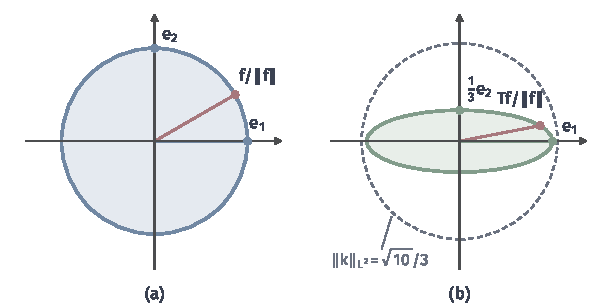
\includegraphics[width=104mm]{figures/04-spaces-measures-and-geometry/03-function-spaces/matplotlib/lop-norm-ellipse/figure.pdf}
  \caption{贯穿例子在$\operatorname{span}\{e_1,e_2\}$上的放大倍数。(a)输入坐标$(\langle e_1,f\rangle,\langle e_2,f\rangle)$中的单位圆（蓝），红点是归一化的$f=1+x$。(b)输出的椭圆（绿），半轴$1$与$1/3$，最长半轴等于$\lVert T\rVert=1$；虚线圆的半径是核的$L^2$范数$\sqrt{10}/3$，它只是上界。}
  \label{fig:lop-norm-ellipse}
\end{BookInlineFigure}

\paragraph{有界算子的矩阵}
到目前为止，矩阵只是类比。在可分Hilbert空间中，有界性让这个类比成为等式。设$H$有标准正交基$(e_n)_{n\geq1}$，$T\in\mathcal B(H)$（记号见下一小节），规定矩阵元素
\begin{equation}
 A_{mn}=\langle e_m,Te_n\rangle .
 \label{eq:lop-matrix-entry}
\end{equation}

任取$x=\sum_nx_ne_n$，部分和$\sum_{n\leq N}x_ne_n$按范数收敛到$x$。由$T$连续，
\[
 Tx=\lim_{N\to\infty}\sum_{n\leq N}x_nTe_n.
\]
再用内积对第二个变量连续，读出第$m$个坐标，就得到矩阵乘法公式
\[
 \langle e_m,Tx\rangle=\sum_nA_{mn}x_n .
\]
连续性在这里不可缺少：它保证算子由基向量上的取值决定。

两个矩阵后面会反复用到。对角算子$A(x_n)=(x_n/n)$在$\ell^2$上的矩阵是$\operatorname{diag}(1,1/2,1/3,\ldots)$；由$\lVert Ax\rVert\leq\lVert x\rVert$及$Ae_1=e_1$得$\lVert A\rVert=1$。右移$S(x_1,x_2,\ldots)=(0,x_1,x_2,\ldots)$的矩阵只在紧贴主对角线下方的一条斜线上为$1$，它保持长度，所以$\lVert S\rVert=1$。

反过来，并非每个无穷矩阵都给出有界算子。对角矩阵$\operatorname{diag}(1,2,3,\ldots)$的放大倍数无界，这是有限维中没有的现象。

\subsection{算子范数的性质}
\label{sec:lop-norm-properties}

同一对空间之间的算子可以相加和数乘：对$S,T:X\to Y$及标量$\alpha$，令$(S+T)x=Sx+Tx$，$(\alpha T)x=\alpha Tx$。若$T:X\to Y$、$S:Y\to Z$，前者的取值空间正是后者的输入空间，就可以复合，$(S\circ T)x=S(Tx)$，常简写为$ST$，先作用$T$、再作用$S$，这对应矩阵乘法。

这些运算都保持线性；下面说明它们也保持有界，并给出范数怎样变化。记$\mathcal B(X,Y)$为定义在整个$X$上、取值于$Y$的有界线性算子全体，$X=Y$时简记$\mathcal B(X)$。

\begin{theorem}[算子范数的基本性质]
\label{thm:lop-norm-properties}
设$X,Y,Z$是赋范空间，$S,T\in\mathcal B(X,Y)$，$R\in\mathcal B(Y,Z)$，$\alpha\in\mathbb F$。则
$\lVert T\rVert\geq0$，且$\lVert T\rVert=0$当且仅当$T=0$；$RT\in\mathcal B(X,Z)$；并且
\begin{equation}
 \begin{gathered}
 \lVert\alpha T\rVert=\lvert\alpha\rvert\,\lVert T\rVert,\qquad
 \lVert S+T\rVert\leq\lVert S\rVert+\lVert T\rVert,\\
 \lVert RT\rVert\leq\lVert R\rVert\,\lVert T\rVert.
 \end{gathered}
 \label{eq:lop-norm-properties}
\end{equation}
因此$\mathcal B(X,Y)$在算子范数下是赋范空间。
\end{theorem}

\begin{proof}
几个估计都先对单个输入成立，再对单位球取上确界。先看正定性。若$\lVert T\rVert=0$，由定理~\ref{thm:lop-norm-minimal}，$\lVert Tx\rVert\leq0$对一切$x$成立，即$T=0$。反之$T=0$时单位球的输出全为零。

数乘由$Y$中范数的齐次性得到：
\[
 \lVert\alpha Tx\rVert=\lvert\alpha\rvert\,\lVert Tx\rVert,
\]
取上确界即得。

加法用$Y$中的三角不等式。对$\lVert x\rVert\leq1$，
\[
 \lVert(S+T)x\rVert\leq\lVert Sx\rVert+\lVert Tx\rVert\leq\lVert S\rVert+\lVert T\rVert.
\]

复合时先用$R$的估计，再用$T$的估计：
\[
 \lVert R(Tx)\rVert_Z\leq\lVert R\rVert\,\lVert Tx\rVert_Y\leq\lVert R\rVert\,\lVert T\rVert\,\lVert x\rVert_X.
\]
这里$Tx$用$Y$的范数衡量，它正是$R$的算子范数所用的输入范数；若$R$的输入范数换成$Y$上的另一个范数，这一步就不能直接衔接。
\end{proof}

复合估计给出多步变换的统一误差上界：输入误差经过$T$至多放大$\lVert T\rVert$倍，再经过$R$至多再放大$\lVert R\rVert$倍。这个上界一般不是等式。在平面上取$\bm T=\operatorname{diag}(1,0)$、$\bm R=\operatorname{diag}(0,1)$，两者的范数都是$1$，乘积却是零矩阵：$\bm T$保留的方向恰好被$\bm R$消去。

\paragraph{算子空间的完备性}
后面要用有限秩算子的极限构造紧算子，对算子级数求和，这需要算子列的极限仍然留在$\mathcal B(X,Y)$中。下面的结论说明，只要取值空间完备，这一点就成立。

\begin{theorem}[算子空间的完备性]
\label{thm:lop-operator-space-complete}
设$X$是赋范空间，$Y$是Banach空间。则$\mathcal B(X,Y)$在算子范数下是Banach空间。
\end{theorem}

\begin{proof}
设$(T_n)$是$\mathcal B(X,Y)$中的柯西列。对固定的$x\in X$，
\[
 \lVert T_nx-T_mx\rVert\leq\lVert T_n-T_m\rVert\,\lVert x\rVert,
\]
所以$(T_nx)$是$Y$中的柯西列。$Y$完备，极限存在，记为$Tx$。由极限的线性，$T$是线性的。

给定$\varepsilon>0$，取$N$使$n,m\geq N$时$\lVert T_n-T_m\rVert<\varepsilon$。对任意$\lVert x\rVert\leq1$及$n\geq N$，有$\lVert T_nx-T_mx\rVert<\varepsilon$。固定$n$而令$m\to\infty$，得
\[
 \lVert T_nx-Tx\rVert\leq\varepsilon\qquad(\lVert x\rVert\leq1,\ n\geq N).
\]

于是$\lVert Tx\rVert\leq\lVert T_N\rVert+\varepsilon$对单位球中的$x$成立，$T$有界。同一估计又说明$\lVert T_n-T\rVert\leq\varepsilon$（$n\geq N$），即$T_n\to T$按算子范数收敛。
\end{proof}

证明只用到了$Y$的完备性，输入空间$X$不必完备。一个直接的用途是：若$T_j\in\mathcal B(X,Y)$且$\sum_j\lVert T_j\rVert<\infty$，则部分和满足
\[
 \Bigl\lVert\sum_{j=m+1}^nT_j\Bigr\rVert\leq\sum_{j=m+1}^n\lVert T_j\rVert,
\]
是柯西列，因而级数$\sum_jT_j$按算子范数收敛。第~\ref{chap:operator-spectra}章用它说明谱的有界性，第~\ref{chap:linear-operator-equations}章再用它构造逆算子。
